\documentclass[10pt,a4paper,twocolumn]{article}
\usepackage[utf8]{inputenc}
\usepackage[T1]{fontenc}
\usepackage[spanish,es-tabla]{babel}
\usepackage[margin=1.8cm,columnsep=0.7cm]{geometry}
\usepackage{graphicx}
\usepackage{amsmath}
\usepackage[hyphens]{url}
\usepackage[hidelinks]{hyperref}
\setlength{\parindent}{1em}
\setlength{\parskip}{0.2em}
\setlength{\emergencystretch}{2em}
\setlength{\textfloatsep}{12pt}
\pagestyle{plain}
\raggedbottom
\renewcommand{\refname}{Referencias}
\newcommand{\pc}[1]{#1\,\%}
\newcommand{\aparef}[1]{\par\noindent\hangindent=1.3em\hangafter=1 #1\par\medskip}
\title{Atribuciones SHAP en MobileNetV3:\\análisis de tres imágenes}
\author{}
\date{}

\begin{document}
\maketitle
\section*{Abstract}
Se analizan las predicciones y los mapas de atribución de MobileNetV3 Small 0.50, variante \texttt{lamb\_in1k}, en tres imágenes: un golden retriever, un cachorro identificado como husky siberiano y una banana. Se examinan las cinco clases con mayor probabilidad y las explicaciones locales obtenidas con \textit{GradientExplainer} de SHAP, mediante 50 muestras y las tres imágenes como referencia. El modelo asignó la primera posición a golden retriever (\pc{86,55}), Eskimo dog (\pc{31,30}) y banana (\pc{69,71}); Siberian husky ocupó la tercera posición (\pc{12,08}) en el segundo caso. Los mapas presentan variaciones visibles en regiones faciales de los perros y un patrón más disperso en la banana, incluido el fondo. La ausencia de color intenso en los contornos no permite afirmar que su contribución sea exactamente cero. El tamaño de la muestra, la referencia compartida, la agregación de canales y la superposición sin invertir el recorte limitan la interpretación espacial. Los resultados ilustran la diferencia entre acertar una etiqueta y obtener una explicación visual localizada, sin establecer mecanismos causales ni rendimiento generalizable.

\noindent\textbf{Palabras clave:} explicabilidad; SHAP; MobileNetV3; clasificación de imágenes.

\section{Introducción}
La clasificación de imágenes mediante redes neuronales permite asignar etiquetas a partir de información visual, pero la clase seleccionada no revela por sí sola qué características contribuyeron a la decisión. En este contexto, las explicaciones locales permiten examinar una predicción concreta y formular hipótesis sobre su relación con la imagen de entrada. Lundberg y Lee (2017) proponen SHAP como un marco de atribución aditiva que asigna contribuciones a las características de una observación.

MobileNetV3 pertenece a una familia de arquitecturas orientadas a equilibrar precisión y costo computacional en dispositivos con recursos limitados (Howard et al., 2019). Este trabajo estudia el modelo preentrenado \texttt{mobilenetv3\_small\_050.lamb\_in1k}, disponible en \textit{timm}, cuya ficha técnica indica entrenamiento en ImageNet-1k (timm, s.\,f.).

El objetivo es describir la correspondencia entre las predicciones de tres casos y sus mapas SHAP: dos perros y una banana. Se examinan la discriminación entre razas caninas, la distribución espacial de las atribuciones y los límites de inferir relevancia a partir del color. El alcance es exploratorio y descriptivo; las tres imágenes no constituyen una evaluación representativa del clasificador.

\section{Metodología}
\subsection{Materiales y clasificación}
La Figura~\ref{fig:entradas} presenta las tres imágenes analizadas. Los archivos de entrada son \texttt{prueba1.jpg}, \texttt{prueba2.jpg} y \texttt{prueba3.jpg}. La primera corresponde a un golden retriever, la segunda a un cachorro descrito como husky siberiano y la tercera a una banana. Estas identidades proceden de la descripción del experimento; no se dispone de una verificación independiente de las razas.

\begin{figure}[tb]
\centering
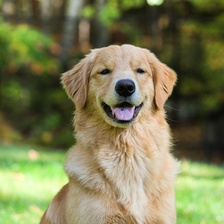
\includegraphics[width=0.315\columnwidth]{images/prueba1.jpg}\hfill
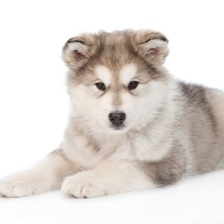
\includegraphics[width=0.315\columnwidth]{images/prueba2.jpg}\hfill
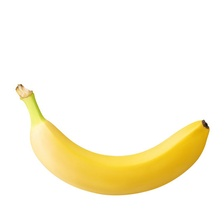
\includegraphics[width=0.315\columnwidth]{images/prueba3.jpg}
\caption{Imágenes de entrada. De izquierda a derecha: prueba 1, golden retriever; prueba 2, cachorro descrito como husky siberiano; prueba 3, banana. Fuente: archivos proporcionados para el experimento.}
\label{fig:entradas}
\end{figure}

El procedimiento se reconstruyó a partir del código y las salidas conservadas en \texttt{main.ipynb}. El modelo se cargó con pesos preentrenados, 1000 clases y modo de evaluación, sin ajuste adicional. La ejecución registrada utilizó CPU y reportó aproximadamente 1,59 millones de parámetros. Las imágenes se convirtieron a RGB y se procesaron mediante la transformación resuelta por \textit{timm}: entrada de $3\times224\times224$, interpolación bicúbica y recorte central con proporción 0,875. La normalización empleó medias $(0,485;0,456;0,406)$ y desviaciones estándar $(0,229;0,224;0,225)$ para los canales RGB.

La salida del modelo es un vector de logits $z(x)$. Para presentar las predicciones se aplicó
\begin{equation}
p_k(x)=\frac{\exp(z_k(x))}{\sum_{j=1}^{1000}\exp(z_j(x))},
\end{equation}
y se seleccionaron las cinco clases de mayor probabilidad. Los porcentajes describen la distribución \textit{softmax} del modelo; no se evaluó su calibración como probabilidades de acierto. Se transcribieron los resultados registrados, sin ejecutar un nuevo experimento de inferencia.

\subsection{Explicación y visualización}
Se empleó \texttt{shap.GradientExplainer}, que aproxima atribuciones SHAP mediante gradientes esperados respecto de un conjunto de referencia (SHAP, s.\,f.). El código utilizó como referencia las tres imágenes preprocesadas y configuró \texttt{nsamples=50} y \texttt{ranked\_outputs=1}. Por tanto, cada mapa explica únicamente la clase ganadora: golden retriever, Eskimo dog o banana. El explicador recibió directamente el modelo, de modo que las atribuciones corresponden a logits, no a los porcentajes posteriores a \textit{softmax}.

Para una clase $k$, el método busca aproximar una descomposición de la diferencia entre su salida y la salida media de referencia:
\begin{equation}
z_k(x)-\mathrm{E}_{b\sim B}[z_k(b)]
\approx \sum_i \phi_i^{(k)}(x),
\end{equation}
donde $B$ es el conjunto de referencia e $i$ recorre las componentes de entrada. La igualdad numérica no se comprobó en los registros disponibles. Las contribuciones se agregaron conservando el signo:
\begin{equation}
H_k(u,v)=\sum_{c\in\{R,G,B\}}\phi_{c,u,v}^{(k)}.
\end{equation}
El mapa se interpoló bilinealmente al tamaño de la imagen original y se representó con una escala simétrica por imagen: rojo para contribuciones positivas y azul para negativas. El límite cromático se fijó en $\max|H_k|+10^{-8}$; por ello, un mismo color no representa necesariamente igual magnitud entre casos.

\subsection{Criterios de interpretación}
La lectura del archivo \texttt{output.png} es cualitativa. Se comparan las zonas de variación cromática con regiones reconocibles del objeto y el fondo. Las atribuciones no son pesos internos del modelo ni mediciones directas de atención. Además, el código redimensiona el mapa sobre la imagen completa sin invertir el recorte central: la correspondencia espacial es aproximada y no permite localizar con precisión anatómica la contribución de cada píxel.

No se conservaron arreglos numéricos de atribución, estimaciones de variabilidad ni versiones de las bibliotecas; tampoco se fijó una semilla en el código. Estas carencias impiden comprobar ceros exactos o estabilidad entre ejecuciones. Las tres imágenes incluyen al propio caso explicado dentro de la referencia, lo que condiciona el contraste y limita su representatividad.

\section{Resultados}
\subsection{Predicciones de las cinco primeras clases}
La Tabla~\ref{tab:resultados} reproduce los quince porcentajes registrados, con sus etiquetas originales. El golden retriever y la banana coinciden con la identidad indicada en la primera posición. En el cachorro, la clase de referencia aparece en tercer lugar. Así, dos de los tres casos coinciden en la primera posición y los tres incluyen la etiqueta indicada entre las cinco primeras; estos conteos no estiman la exactitud poblacional del modelo.

\begin{table}[tb]
\centering
\caption{Cinco clases con mayor probabilidad por imagen.}
\label{tab:resultados}
\small
\begin{tabular}{cl r}
\hline
Prueba & Clase & Probabilidad \\
\hline
1 & golden retriever & \pc{86,55} \\
  & Labrador retriever & \pc{1,80} \\
  & kuvasz & \pc{1,40} \\
  & Norfolk terrier & \pc{1,18} \\
  & Rhodesian ridgeback & \pc{0,44} \\
\hline
2 & Eskimo dog & \pc{31,30} \\
  & malamute & \pc{25,87} \\
  & Siberian husky & \pc{12,08} \\
  & Arctic fox & \pc{5,50} \\
  & collie & \pc{2,01} \\
\hline
3 & banana & \pc{69,71} \\
  & spaghetti squash & \pc{5,40} \\
  & sunglass & \pc{1,05} \\
  & lemon & \pc{1,01} \\
  & whistle & \pc{0,79} \\
\hline
\end{tabular}
\par\smallskip
\begin{minipage}{\columnwidth}\footnotesize
\textit{Nota.} Valores \textit{softmax} conservados en el cuaderno, redondeados a dos decimales. Las cinco filas de cada caso no suman el 100\,\% porque se omiten las otras 995 clases.
\end{minipage}
\end{table}

En la prueba 1, la diferencia entre golden retriever y Labrador retriever es de 84,75 puntos porcentuales. En la prueba 2, Eskimo dog supera a malamute por solo 5,43 puntos; Siberian husky alcanza \pc{12,08}. Las tres primeras etiquetas son razas de perros y reúnen \pc{69,25}. Este resultado es compatible con una identificación canina amplia, pero no equivale a acertar la raza ni constituye una probabilidad agregada exhaustiva de la categoría perro.

En la prueba 3, banana obtiene \pc{69,71}, frente a \pc{5,40} de spaghetti squash: una diferencia de 64,31 puntos porcentuales. La separación entre las dos primeras clases es mayor que en el cachorro. Estas diferencias describen la concentración de la salida en cada caso, sin demostrar robustez ante nuevas imágenes o perturbaciones.

\begin{figure*}[t]
\centering
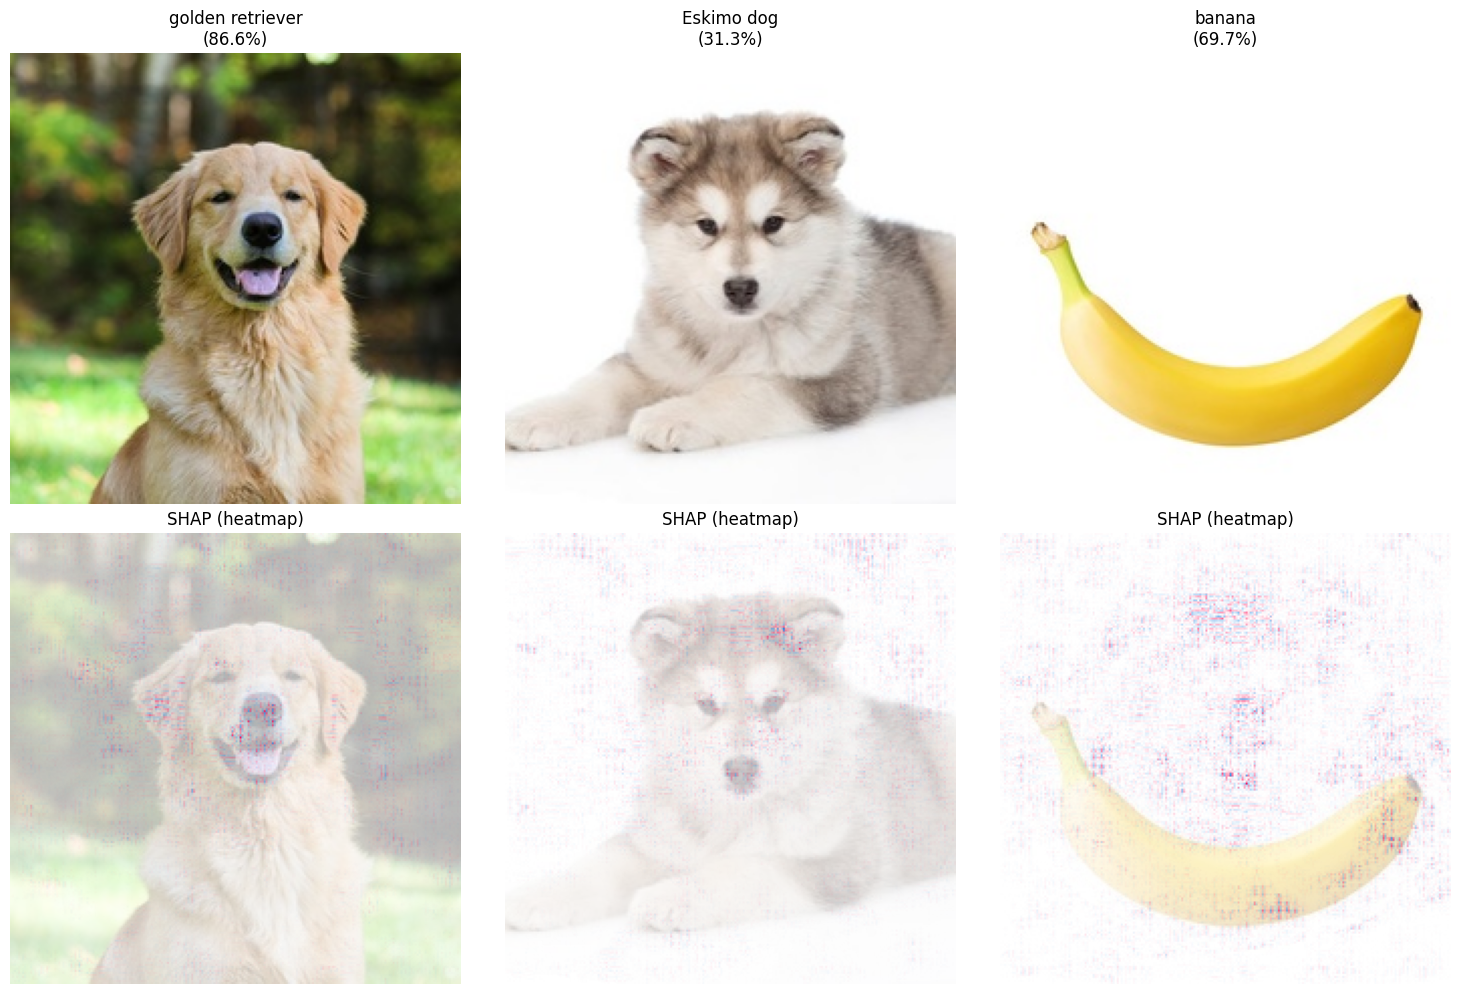
\includegraphics[width=0.91\textwidth]{images/output.png}
\caption{Predicciones y mapas SHAP proporcionados. Columnas: golden retriever, cachorro y banana. La fila inferior explica el logit de la clase ganadora indicada en la fila superior; en el cachorro corresponde a Eskimo dog. Rojo y azul representan contribuciones positivas y negativas, respectivamente, con escala independiente por imagen. La superposición no invierte el recorte central del preprocesamiento, por lo que su alineación es aproximada. Fuente: \texttt{images/output.png}, asociado al procedimiento de \texttt{main.ipynb}.}
\label{fig:shap}
\end{figure*}

\subsection{Distribución visual de las atribuciones}
En el golden retriever, la Figura~\ref{fig:shap} muestra variación roja y azul en torno al hocico y la nariz, así como cerca de las orejas. En el cachorro se distinguen contribuciones en regiones próximas a la frente, las orejas, los ojos y la nariz. Estas coincidencias sugieren participación de información facial en las salidas explicadas, con la cautela de alineación descrita. Sin una cuantificación por regiones, no puede establecerse que esas áreas acumulen la mayor contribución total. Tampoco todos los colores sobre el rostro favorecen la clase: los azules indican contribuciones negativas.

Los mapas no delinean de manera continua la silueta de los perros. Esta observación se expresa como escasa señal cromática visible del contorno, y no como contribución exactamente nula. La suma de canales puede cancelar valores de signo opuesto; además, la escala y la transparencia pueden ocultar contribuciones pequeñas. Incluso un valor agregado igual a cero no demostraría que la forma carezca de utilidad para el modelo.

En la banana aparece un patrón más disperso, con contribuciones visibles tanto en el fruto como en el fondo, especialmente en la zona superior central. No se observa un trazado continuo del borde ni un foco visual inequívoco en el tallo o las líneas longitudinales. La apariencia irregular no demuestra aleatoriedad: no se aplicó una prueba estadística ni se contrastó con otras referencias. La clasificación correcta coexiste, en este caso, con una explicación menos localizada en partes reconocibles del objeto.

\subsection{Alcance de los hallazgos}
El mapa del cachorro explica la puntuación de Eskimo dog; no explica directamente por qué dicha clase supera a Siberian husky o malamute. Para estudiar esa confusión sería necesario comparar atribuciones de las tres clases o explicar sus diferencias de logits. La semejanza visual entre razas es una hipótesis compatible con el resultado, pero no una causa verificada por este análisis.

Asimismo, la señal sobre el fondo de la banana plantea una posible dependencia del contexto, aunque no permite confirmarla. El uso de imágenes caninas como parte de la referencia y la superposición aproximada también pueden influir en su apariencia. Harían falta intervenciones controladas sobre el fondo y la conservación de los valores numéricos para distinguir estas posibilidades.

\section{Conclusiones}
El análisis de tres imágenes muestra coincidencia entre la etiqueta indicada y la primera predicción para el golden retriever y la banana. El cachorro descrito como husky siberiano fue clasificado como Eskimo dog, seguido de malamute y Siberian husky, lo que evidencia una confusión de raza dentro de las primeras opciones caninas.

Los mapas permiten identificar variaciones de atribución próximas a rasgos faciales de los perros y una distribución más dispersa para la banana. Sin embargo, ni la falta de un contorno coloreado prueba una contribución exactamente cero ni una predicción correcta garantiza una explicación concentrada sobre el objeto. Las conclusiones son locales y están condicionadas por la referencia, el muestreo, la agregación de canales y la alineación espacial.

Para fortalecer el estudio se propone ampliar la muestra, usar referencias independientes y diversas, fijar semillas y versiones, repetir las explicaciones y guardar sus arreglos numéricos. También conviene representar los mapas sobre la entrada efectivamente recortada, compartir una escala de magnitud y cuantificar atribuciones por regiones junto con pruebas de perturbación. Estas extensiones permitirían evaluar estabilidad y dependencia del contexto antes de formular afirmaciones generales sobre el comportamiento del modelo.

\section*{Referencias}
\begingroup
\small
\raggedright
\aparef{Howard, A., Sandler, M., Chu, G., Chen, L.-C., Chen, B., Tan, M., Wang, W., Zhu, Y., Pang, R., Vasudevan, V., Le, Q. V., \& Adam, H. (2019). Searching for MobileNetV3. En \textit{Proceedings of the IEEE/CVF International Conference on Computer Vision} (pp. 1314--1324). \url{https://doi.org/10.1109/ICCV.2019.00140}}
\aparef{Lundberg, S. M., \& Lee, S.-I. (2017). A unified approach to interpreting model predictions. En I. Guyon, U. von Luxburg, S. Bengio, H. Wallach, R. Fergus, S. Vishwanathan y R. Garnett (Eds.), \textit{Advances in neural information processing systems} (Vol. 30). Curran Associates, Inc. \url{https://papers.nips.cc/paper/7062-a-unified-approach-to-interpreting-model-predictions}}
\aparef{SHAP. (s.\,f.). \textit{shap.GradientExplainer} [Documentación de software]. Recuperado el 4 de septiembre de 2026, de \url{https://shap.readthedocs.io/en/latest/generated/shap.GradientExplainer.html}}
\aparef{timm. (s.\,f.). \textit{mobilenetv3\_small\_050.lamb\_in1k} [Ficha de modelo]. Hugging Face. Recuperado el 4 de septiembre de 2026, de \url{https://huggingface.co/timm/mobilenetv3_small_050.lamb_in1k}}
\endgroup
\end{document}
